%\documentclass{beamer}
%\documentclass[handout]{beamer}
%\documentclass[12pt,handout]{beamer}
\documentclass[12pt,donthandout,notes=dontshow,xcolor=table]{beamer}

\NeedsTeXFormat{LaTeX2e}
\usepackage[orientation=landscape,size=custom,width=16,height=9,scale=.5,debug]{beamerposter} 
\usepackage[utf8]{inputenc}
%\usepackage[german]{babel}

\usepackage{tcolorbox}

%\usepackage[table]{xcolor}
%\usepackage{tabularx}
%\usepackage{textcomp}
%\usepackage{tikz}
%\usetikzlibrary{shapes,arrows,positioning,trees,shadings,decorations.pathreplacing,backgrounds}
%\usepackage{tcolorbox}
%\usepackage{pdfpages}
%\usepackage{listings}
%\usepackage{longtable}
%
%\usepackage{minted}

%\usetheme{Madrid}
\usetheme{Goettingen}

%%%%%%%%%%% PRINT NOTES
%\usepackage{pgfpages}
%\pgfpagesuselayout{2 on 1}[a4paper]
%\setbeameroption{show notes on second screen=bottom} % Beamer manual, section 19.3
%\usetemplatenote{\beamertemplatefootempty \insertnote}
%%%%%%%%%%% PRINT NOTES

%\useoutertheme{shadow}
%\setbeamertemplate{items}[default]
\beamertemplatenavigationsymbolsempty
\setbeamertemplate{footline}[frame number]

\author{Sebastian Bernauer}
\title[Pixelflut v6]{Pixelflut v6\\As fast as possible?}

%\AtBeginSection[]
%{
%	\begin{frame}{Inhalt}
%	\tableofcontents[currentsection]
%	\end{frame}
%}

\begin{document}
\begin{frame}
\titlepage
\end{frame}

\begin{frame}%[allowframebreaks]
\frametitle{Inhalt}
\tableofcontents
\end{frame}

\section{Bestandsaufnahme}

\subsection{Pixelflut (v4)}
\begin{frame}{Pixelflut (v4)}
	\begin{itemize}
		\item ASCII-Befehle über TCP, Zeile für Zeile
	\end{itemize}
	\vfill
	\begin{tcolorbox}[title=Verwendung]
	echo "PX x y rrggbb[aa]" $\vert$ nc 127.0.0.1 1234
	\end{tcolorbox}
\end{frame}

\begin{frame}{Software}
	\begin{itemize}
		\item Server: shoreline von TobleMiner
		\begin{itemize}
			\item 37G mit Dual AMD EPYC (!)
			\item https://github.com/TobleMiner/shoreline
		\end{itemize}
		\pause
		\item Client: sturmflut
		\begin{itemize}
			\item 80G mit Laptop
			\item https://github.com/TobleMiner/sturmflut
		\end{itemize}
	\end{itemize}
	\pause
	\begin{tcolorbox}[title=Problem]
	Ein Client macht Server locker platt
	\end{tcolorbox}
\end{frame}

\subsection{Pixelflut v6}
\begin{frame}[fragile]{Pixelflut v6}
	Das Format der zu sendenden IPv6-Adresse:
	\begin{itemize}
	\item 64 bit festes Prefix
	\item    16 bit X-Koordinate
	\item    16 bit Y-Koordinate
	\item    8 bit R
	\item    8 bit G
	\item    8 bit B
	\item    8 bit Padding
	\end{itemize}
	
	Gesamt ergibt sich: \texttt{Prefix:XXXX:YYYY:RRGG:BBPP}
\end{frame}

\begin{frame}{Beispiel}
	\begin{tcolorbox}[title=Beispiel]
	ping 4000:42:0:0:0505:ffaa:ccff\\
	\begin{itemize}
		\item Netz: 4000:42::/64
		\item X = 5
		\item Y = 5
		\item Farbe: 0xffaacc
	\end{itemize}
	\end{tcolorbox}
\end{frame}

\begin{frame}{Implikationen}
	\begin{itemize}
		\item Ganz viele kleine Packete
		\pause
		\item Use moare bandwith as pixelflut v4 :)\\
		\texttt{"PX 123 123 rrggbb{\textbackslash}n}" (18 byte) \\vs \\$\ge$ 64 byte Packet
		\item Linux kernel kommt an seine Grenzen
	\end{itemize}
\end{frame}

\begin{frame}{Software}
	\begin{itemize}
		\item Server: ?
		\pause
		\item Client: ?
		\pause
		\item Selber machen!
	\end{itemize}
\end{frame}

\section{Architektur}
\begin{frame}{Architektur}
	\begin{itemize}
		\item Üblicher Weg: Linux Kernel und C-Programm\\
		$\rightarrow$ Wie shoreline\\
		$\rightarrow$ Problem: Packete/s im Kernel
		\pause
		\item FPGA\\
		$\rightarrow$ Cool\\
		$\rightarrow$ Problem: Teuer
		\pause
		\item XDP (Express Data Path)\\
		$\rightarrow$ Programm läuft direkt im Linux kernel\\
		$\rightarrow$ Kein Kopieren in userspace nötig\\
		$\rightarrow$ Keine Kontextwechsel nötig
	\end{itemize}
\end{frame}

\begin{frame}{Architektur}
	\begin{itemize}
		\item DPDK (Data Plane Development Kit)\\
		$\rightarrow$ Netzwerkkarte wird komplett im userspace angesprochen\\
		$\rightarrow$ Keine Interrupts, sondern Poll basiert
	\end{itemize}
\end{frame}

\begin{frame}{XDP}
	\begin{itemize}
		\item Hat wunderbar funktioniert
		\item Pixelinformationen wurden in einer Datenstruktur im Kernel abgelegt
		\item Für das Erfragen eines Elementes der Datenstruktur\\
		$\rightarrow$ Alle Pixel aus Datenstruktur lesen: 2s\\
		\hspace{1cm} $\rightarrow$ 1920 x 1080 = 2.073.600 System calls! \\
		$\rightarrow$ Nix da mit 60 fps
		\item Läuft auf jeder Netzwerkkarte
	\end{itemize}
	\pause
	\begin{tcolorbox}[title=Problem]
		Wir kriegen die Daten nicht aus der Datenstruktur im Kernel
	\end{tcolorbox}
\end{frame}

\begin{frame}{XDP}
	Möglichkeiten zur Lösung des Problems
	\begin{itemize}
		\item Kernel contribution: Komplette Datenstruktur mit einem Systemcall aus dem Kernel in den userspace kopieren
		\pause
		\item \textbf{Achtung abgespaced:}
		\pause
		\item Man kann in XDP Packete manipulieren und an den Absender zurück senden.\\
		$\rightarrow$ Server empfängt alle Pixel-Packete und aktualisiert Datenstruktur im Kernel\\
		$\rightarrow$ Client erzeugt einen konstanten Strom um 60fps rendern zu rendern, in einem Packet wird mittels Offset und Länge nach Pixelwerten gefragt\\
		$\rightarrow$ Server modifiziert Packet (welches richtige Länge hat ;)) mit den gewünschten Pixeln und schickt es an den Absender zurück (In diesem Shritt kann auf Datenstruktur zugegriffen werden)\\
		$\rightarrow$ Keine Modifikation am Kernel notwendig
	\end{itemize}
\end{frame}

\section{Netzarchitektur}
\begin{frame}{Netzarchitektur}
	\begin{itemize}
		\item Neighbor Discovery von $>$ 2 Millionen IPv6 Adressen (Full HD)?\\
		\pause
		$\rightarrow$ Nein!
	\end{itemize}
\end{frame}

\begin{frame}{Netzarchitektur}
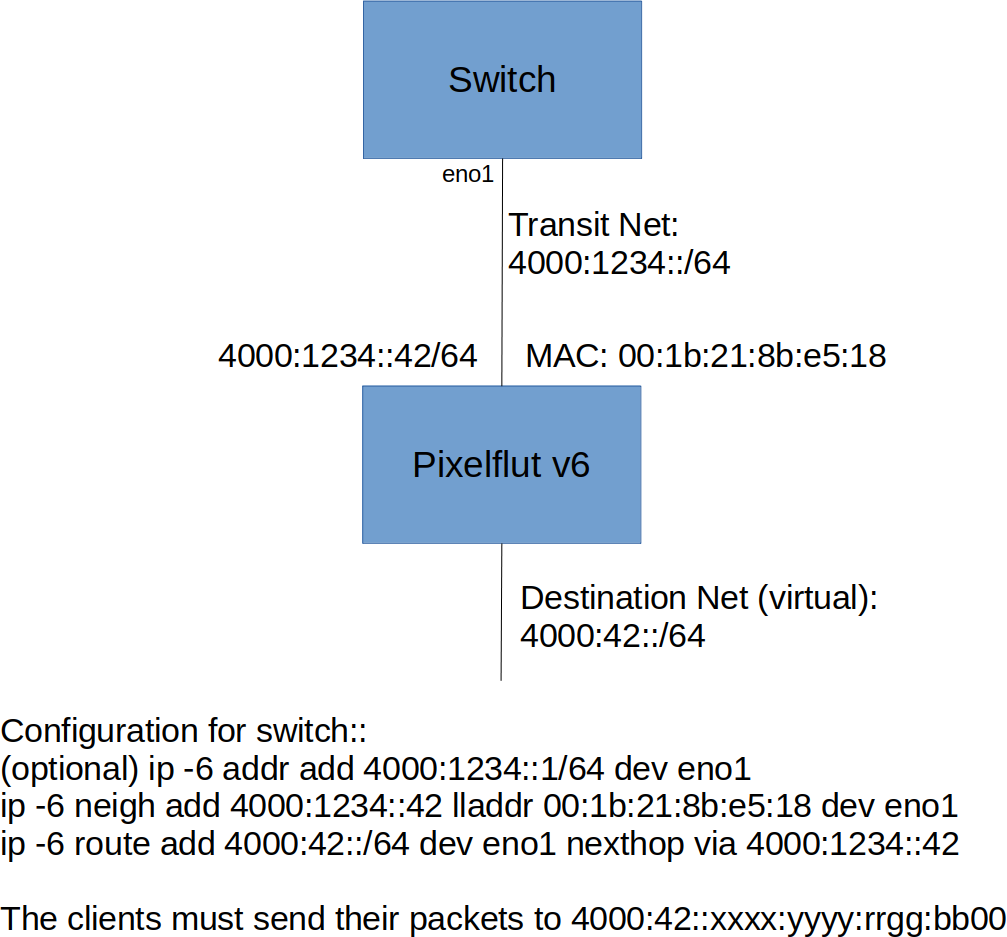
\includegraphics[width=8cm]{figures/network_structure_cut}
\end{frame}

\end{document}